\section{Evaluation} %%%%%%%%%%%%%%%%%%%%%%%%%%%%%%%%%%%%%%%%%%%%%%%%%%%%%%%%%%%
\label{sec:eval}

We performed several independent studies of our pattern matching solution to 
test its efficiency and impact on compilation process. In the first study we 
compare various functions written with pattern matching and hand-optimized 
manually in order to estimate the overhead added by the composition of patterns 
(\textsection\ref{sec:patcmp}). We demonstrate this overhead for both our 
solution based on compile-time composition of patterns and the suggested 
alternatives based on the run-time composition of patterns. In the second 
study we compare a relevant impact on the compilation times brought by both 
approaches (\textsection\ref{sec:ctcmp}). In the third study, we looked at how well our extension 
of \code{Match}-statement to $N$-arguments using the Morton order deals with 
large real-world class hierarchies (\textsection\ref{sec:morton}). In the third 
study we compare the performance of matching $N$ polymorphic arguments against 
double, triple and quadruple dispatch via visitor design pattern as well as 
open multi-methods extension to \Cpp{} (\textsection\ref{sec:dd}). 
In the last study, we rewrote a code 
optimizer of an experimental language from Haskell into \Cpp{} with 
\emph{Mach7}. We compare the ease of use, readability and maintainability 
of the original Haskell code and its \emph{Mach7} equivalent 
(\textsection\ref{sec:qualcmp}).

The studies involving performance comparisons have been performed on 
Sony VAIO\textsuperscript{\textregistered} laptop with 
Intel\textsuperscript{\textregistered} Core\texttrademark i5 460M CPU at 2.53 
GHz; 6GB of RAM; Windows 7 Professional. All the code was compiled with G++ 
(versions 4.5.2, 4.6.1 and 4.7.2; executed with -O2 to produce x86 binaries 
under MinGW) as well as Visual \Cpp{} (versions 10.0 and 11.0 with 
profile-guided optimizations enabled).
 
To improve accuracy, timing was performed with the help of \code{RDTSC} 
instruction available on x86 processors. For every number reported we ran 
101 experiments timing 1,000,000 top-level calls each (depending on arguments, 
there may have been a different number of recursive calls). The first experiment 
was serving as a warm-up, and typically resulted in an outlier with the largest 
time. Averaged over 1,000,000 calls, the number of cycles per top-level call in 
each of the 101 experiments was sorted and the median was chosen. We preferred 
median to average to diminish the influence of other applications and OS 
interrupts as well as to improve reproducibility of timings between the runs of 
application. In particular, in the diagnostic boot of Windows, where the minimum 
of drivers and applications are loaded, we were getting the same number of 
cycles per iteration 70-80 out of 101 times. Timings in non-diagnostic boots had 
somewhat larger absolute values, however the relative performance remained 
unchanged and equally well reproducible.

\subsection{Pattern Matching Overhead}
\label{sec:patcmp}

The overhead associated with pattern matching may originate from several 
different sources:

\begin{itemize}
\setlength{\itemsep}{0pt}
\setlength{\parskip}{0pt}
\item Naive (sequential and often duplicated) order of tests due to a pure 
      library solution. 
\item Compiler's inability to inline the test expressed by the pattern in the 
      left-hand side of the case clause (e.g. due to lack of [type] information 
      or complexity of the expression). 
\item Compiler's inability to elide construction of pattern trees when used in 
      the right-hand side of the case clause.
\end{itemize}

\noindent
To estimate the overhead introduced by commonly used \emph{patterns as objects} 
approach (\textsection\ref{sec:pao}) and our \emph{patterns as expression 
templates} approach (\textsection\ref{sec:pat}), we implemented several simple
functions with and without pattern matching. The handcrafted code we compared 
against was hand-optimized by us to render the same results, without changes to 
the underlying algorithm. Some functions were implemented in several ways with 
different patterns in order to show the impact of different patterns and pattern 
combinations on performance. The overhead of both approaches on a range of 
recent \Cpp{} compilers is shown in Figure~\ref{fig:overhead}.

\begin{figure}[htbp]
\scriptsize
\begin{tabular}{|@{}l@{}|@{}l@{}||@{}r@{}|@{}r@{}|@{}r@{}|@{}r@{}|@{}r@{}||@{}r@{}|@{}r@{}|@{}r@{}|@{}r@{}|@{}r@{}|}
\hline % ------------------------------------------------------------------
             &           & \multicolumn{5}{@{}c@{}||}{Patterns as Expr. Templates}
                         & \multicolumn{5}{@{}c@{}|}{Patterns as Objects} \\
\hline % ------------------------------------------------------------------
             &           & \multicolumn{3}{@{}c@{}|}{G++} & \multicolumn{2}{@{}c@{}||}{Visual C++}
                         & \multicolumn{3}{@{}c@{}|}{G++} & \multicolumn{2}{@{}c@{}|}{Visual C++} \\
\hline % ------------------------------------------------------------------
Test         & Patterns  &  4.5.2 &  4.6.1 &  4.7.2 &   10.0 &   11.0 &  4.5.2 &  4.6.1 &  4.7.2 &   10.0 &   11.0  \\ % & NLOC$_h$ & NLOC$_p$
\hline % -------------------------------------------------------------------------------------------------  % Diagnostic boot timings from 2013-03-10
factorial$^*_0$& 1,v,\_  & \f{15} & \f{13} & \f{17} &\s{ 85} &\s{ 35} &\s{ 347}&\s{ 408}&\s{ 419}&\s{2121}&\s{1788} \\ % &        6 &        7
factorial$_1$& 1,v       & \s{ 0} & \s{ 6} & \s{ 0} &\s{ 83} &\s{ 21} &\s{ 410}&\s{ 519}&\s{ 504}&\s{2380}&\s{1812} \\ % &        6 &        7
factorial$_2$& 1,n+k     & \s{ 7} & \s{ 9} & \s{ 6} &\s{ 78} &\s{   } &\s{ 797}&\s{ 911}&\s{ 803}&\s{3554}&\s{3057} \\ % &          &         
fibonacci$^*$& 1,n+k     & \s{17} & \f{ 2} & \s{ 2} &\s{ 62} &\s{ 15} &\s{ 340}&\s{ 431}&\s{ 395}&\s{2730}&\s{2597} \\ % &        7 &        8
gcd$^*_1$    & v,n+k,+   & \s{21} & \s{25} & \s{25} &\s{309} &\s{179} &\s{1503}&\s{1333}&\s{1208}&\s{8876}&\s{7810} \\ % &        6 &        7
gcd$_2$      & 1,n+k,\_  & \s{ 5} & \s{13} & \s{19} &\s{373} &\s{303} &\s{ 962}&\s{1080}&\s{ 779}&\s{5332}&\s{4674} \\ % &        6 &        7
gcd$_3$      & 1,v       & \f{ 1} & \s{ 0} & \f{ 1} &\s{ 38} &\s{ 15} &\s{ 119}&\s{ 102}&\s{ 108}&\s{1575}&\s{1319} \\ % &        6 &        7
lambdas$^*$  & \&,v,C,+  & \s{58} & \s{54} & \s{56} &\f{ 29} &\f{ 34} &\s{ 837}&\s{ 780}&\s{ 875}&\s{ 259}&\s{ 289} \\ % &       15 &       10
power        & 1,n+k     & \s{10} & \s{ 8} & \s{13} &\s{ 50} &\s{  6} &\s{ 291}&\s{ 337}&\s{ 338}&\s{1950}&\s{1648} \\ % &        9 &        8
balance$^*$  & 1,v,C     & \s{  } & \s{  } & \s{  } &\s{   } &\s{   } &\s{    }&\s{    }&\s{    }&\s{    }&\s{    } \\ % &          &       10
\hline % ------------------------------------------------------------------
\end{tabular}
\caption{Pattern Matching Overhead}
\label{fig:overhead}
\end{figure}

%
%Figure~\ref{fig:overhead} lists several functions we compared, the kinds of 
%patterns that were involved in the pattern-matching implementation of them, the 
%overhead our implementation as well as implementation in patterns-as-objects 
%approach had over the hand crafted implementation. We also list the number of 
%non-empty lines of code corresponding functions of handcrafted, our approach 
%and patterns-as-objects approach had. 

The experiments marked with $*$ correspond to the code of their respective 
functions shown in \textsection\ref{sec:cpppat}. The rest of the functions, 
including all the implementations with ``patterns as objects'' approach, are 
available among the files accompanying this submission and will be made 
available later on the project's web page. The patterns involved in each 
experiment are abbreviated as following:

%\begin{figure}[htb]
%  \centering
%  \scriptsize
\begin{center}
  \begin{minipage}[t]{0.45\linewidth}
      {\bf 1}  -- value pattern    \\
      {\bf v}  -- variable pattern \\
      {\bf \_} -- wildcard pattern
  \end{minipage}
  \begin{minipage}[t]{0.45\linewidth}
      {\bf n+k} -- n+k pattern            \\
      {\bf +}   -- equivalence combinator \\
      {\bf \&}  -- address combinator     \\
      {\bf C}   -- constructor pattern   
  \end{minipage}
\end{center}
%\end{figure}

\noindent
It is easy to see that the overhead incurred by compile-time composition of 
patterns in \emph{patterns as expression templates} approach is significantly 
smaller than the overhead of run-time composition of patterns in \emph{patterns 
as objects} approach. In fact, in several cases, shown in the table in bold 
font, the compiler was able to eliminate the overhead entirely and even generate 
a faster code. In case of ``lambdas'' experiment, the advantage was mainly due 
to the underlying type switch, while in the rest of the cases the generated code
was feeding better the instruction pipeline and the branch predictor.

In each experiment, the handcrafted baseline implementation was the same in 
both cases (compile-time and run-time composition) and reflected our idea of the 
fastest code without pattern matching describing the same algorithm. For 
example, gcd$_3$ was implementing the fast Euclidian algorithm with remainders, 
while gcd$_1$ and gcd$_2$ were implementing its slower version with 
subtractions. The baseline code was correspondingly implementing fast Euclidian 
algorithm for gcd$_3$ and slow for gcd$_1$ and gcd$_2$.

The comparison of the overhead incurred by both approaches would be incomplete 
without detailing the implementation of patterns as objects solution. In particular, 
dealing with objects in object-oriented languages often involves heap allocation, 
subtype tests, garbage collection etc., which all can significantly affect the 
performance. To make this comparison applicable to a wider range of 
object-oriented languages, we took the following precautions in the 
``objects as patterns'' implementations:

\begin{itemize}
\setlength{\itemsep}{0pt}
\setlength{\parskip}{0pt}
\item All the objects involved were stack-allocated or statically allocated. 
      This measure was taken to avoid allocating objects on the heap, which is 
      known to be much slower and is an optimization compilers of many 
      object-oriented languages undertake.
\item Objects representing constant values as well as patterns whose state 
      does not change during pattern matching (e.g. wildcard and value patterns) 
      were all statically allocated.
\item Patterns that modify their own state were constructed only when they were 
      actually used, since a successful match by a previous pattern may return 
      early from the function.
\item Only the arguments on which pattern matching was effectively performed 
      were boxed into the \code{object} class hierarchy, e.g. in case of power 
      function only the second argument was boxed.
\item Boxed arguments were statically typed with their most derived type to 
      avoid unnecessary type checks and conversions: e.g. \code{object_of<int>&}, 
      which is a class derived from \code{object} to represent a boxed integer, 
      instead of just \code{object&}.
\item No objects were returned as a result of a function as in truly 
      object-oriented approach that would typically require heap allocation.
\item n+k patterns that effectively require evaluating a result of an expression 
      where implemented with an additional virtual function instead that simply
      checks whether a result is a given value. This does not allow expressing
      all n+k patterns of \emph{Mach7}, but was sufficient to express all those 
      involved in the experiments and allowed us to avoid heap allocating the 
      results. 
\item When run-time type checks were unavoidable (e.g. inside \code{pattern::match} 
      implementation) we were comparing type-ids first, and only when the 
      comparison failed were invoking the dynamic cast. This typical 
      optimization avoids the much slower dynamic cast in the common case.
\end{itemize}

\noindent
With these precautions in place, we believe that the main overhead of the 
patterns-as-objects solution that we were measuring was in the cost of a virtual 
function call (\code{pattern::match}) and the cost of run-time type 
identification and conversion on its argument -- the subject. Both are specific 
to the approach and not to our implementation of it, which is why we believe a 
similar overhead will be present in other object-oriented languages following 
this strategy to pattern matching.

\subsection{Compilation Time Overhead}
\label{sec:ctcmp}

Several people expressed their concerns about possible significant increase in 
the compilation time due to opennes of our pattern matching solution. To 
disperse these worries we compared relative increase or decrease of compilation 
time for each of the examples discussed in \textsection\ref{sec:patcmp}. 
We slightly modified each code to only compile either the hand-crafted version 
or the pattern-matching one. We removed the definition of the unused function in 
each case, however we kept the set of included headers unchanged to avoid 
affecting of overal timing by the time spent in the parser. We then measured the 
time spent in the compilation phase of the compiler and report the percentage 
increase of the slower one against the faster one. Each compilation time has 
been measure 3 times and the median was used in the actual comparison.

\begin{table}[htbp]
\centering
\scriptsize
\begin{tabular}{|@{}l@{}|@{}l@{}||@{}r@{}|@{}r@{}|@{}r@{}||@{}r@{}|@{}r@{}|@{}r@{}|}
\hline % ------------------------------------------------------------------
             &           & \multicolumn{3}{@{}c@{}||}{Open Patterns}
                         & \multicolumn{3}{@{}c@{}|}{Patterns as Objects} \\
\hline % ------------------------------------------------------------------
             &           & \multicolumn{1}{@{}c@{}|}{G++} & \multicolumn{2}{@{}c@{}||}{Visual C++}
                         & \multicolumn{1}{@{}c@{}|}{G++} & \multicolumn{2}{@{}c@{}|}{Visual C++} \\
\hline % ------------------------------------------------------------------
Test         & Patterns  &     4.7.2 &    10.0 &     11.0 &   4.7.2 &    10.0 &    11.0  \\ % & NLOC$_h$ & NLOC$_p$
\hline % -------------------------------------------------------------  % Timing-Compilation.xlsx
factorial$^*_0$& 1,v,\_  & \s{ 1.65} &\s{1.65} &\s{ 2.95} &\s{ 7.10}&\f{10.00}&\s{10.68} \\ % &        6 &        7
factorial$_1$& 1,v       & \s{ 2.46} &\s{1.60} &\s{10.92} &\s{ 7.14}&\s{ 0.00}&\s{ 1.37} \\ % &        6 &        7
factorial$_2$& 1,n+k     & \s{ 2.87} &\s{3.15} &\s{ 3.01} &\s{ 8.93}&\s{ 4.05}&\f{ 3.83} \\ % &          &         
fibonacci$^*$& 1,n+k     & \s{ 3.66} &\s{1.60} &\s{ 2.95} &\s{11.31}&\f{ 4.03}&\s{ 1.37} \\ % &        7 &        8
gcd$^*_1$    & v,n+k,+   & \s{ 4.07} &\s{4.68} &\f{ 0.91} &\s{ 9.94}&\s{ 2.05}&\s{ 8.05} \\ % &        6 &        7
gcd$_2$      & 1,n+k,\_  & \s{ 1.21} &\s{1.53} &\f{ 0.92} &\s{ 8.19}&\f{ 2.05}&\f{ 2.58} \\ % &        6 &        7
gcd$_3$      & 1,v       & \s{ 2.03} &\s{3.15} &\s{ 7.86} &\s{ 5.29}&\s{ 2.05}&\s{ 0.08} \\ % &        6 &        7
lambdas$^*$  & \&,v,C,+  & \s{18.91} &\s{7.25} &\f{ 4.27} &\s{ 4.57}&\f{ 3.82}&\s{ 0.00} \\ % &       15 &       10
power        & 1,n+k     & \s{ 2.00} &\s{6.40} &\s{ 3.92} &\s{ 8.14}&\s{ 0.13}&\s{ 4.02} \\ % &        9 &        8
%balance$^*$ & 1,v,C     & \s{}      &\s{}     &\s{}      &\s{     }&\s{     }&\s{     } \\ % &          &       10
\hline % ------------------------------------------------------------------
\end{tabular}
\caption{Compilation Time Overhead}
\label{tbl:ctoverhead}
\end{table}

As can be seen in Table~\ref{tbl:ctoverhead}, most of the time the hand-crafted 
code was compiling faster (entries indicated with regular font), however in few 
cases the pattern-matching code was compiling faster (entries indicated in bold 
font). In any case the difference in compilation times was not significant -- on 
average 3.99\% for open patterns and 4.84\% for patterns as objects. Bear in 
mind that we were compiling relatively small files with only difference in a 
single function and that the difference on real-world projects with significant 
percentage of non-pattern matching code will be even less noticable.

\subsection{Multi-argument Hashing}
\label{sec:morton}

To check the efficiency of hashing in the multi-argument \code{Match}-statement 
(\textsection\ref{sec:matchstmt}) we used the same class hierarchy benchmark we 
used to test the efficiency of hashing in type switch~\cite[\textsection 4.4]{TS12}.
The benchmark consists of 13 libraries describing 15246 classes totally. Not all 
the class hierarchies originated from \Cpp{}, but all were written by humans and 
represent actual relationships in their problem domains.

While \code{Match}-statement works with both polymorphic and non-polymorphic 
arguments, only the polymorphic arguments are taken into consideration for 
efficient type switching and thus efficient hashing. It also generally makes 
sense to apply type switching to non-leaf nodes of the class hierarchy only. 71\%
of the classes in the entire benchmarks suite were leaf classes. For each of the 
remaining 4369 non-leaf classes we created 4 functions, performing case analysis 
on derived class on a combination of 1, 2, 3 and 4 arguments respectively. Each 
of the functions was executed with different combinations of possible derived 
types, including, in case of repeated multiple inheritance, different 
sub-objects within the same type. There was 63963 different subobjects when the 
class hierarchies used repeated multiple inheritance and 38856 different 
subobjects when the virtual multiple inheritance was used.

As with type switching, for each of the 4369 functions (per same number of 
arguments) we were measuring the number of conflicts $m$ in cache -- the number 
of entries mapped to the same location in cache by the optimal hash function. 
We then computed the percentage of functions that achieved a given number of 
conflicts, which we show in Figure~\ref{fig:hashing}.

% NOTE: Data from 2013-02-24, see ClassHierarchiesMultipleArguments-2013-02-20.xlsx
\begin{figure}[htbp]
\small
\begin{tabular}
{@{}c@{ }|@{}c@{}||@{ }r@{}|@{ }r@{}|@{ }r@{}|@{ }r@{}|@{ }r@{}|@{ }r@{}|@{ }r@{}}
\hline % -------------------------------------------------------------------------
\multicolumn{2}{@{}c@{}||}{$N/m$} & [0] & [1] & $\cdots$ 10] & $\cdots$ 100] & $\cdots$ 1000] & $\cdots$ 10000] & \textgreater 10000 \\
\hline % -------------------------------------------------------------------------
\multirow{4}{*}{\begin{sideways}{\scriptsize Repeated}\end{sideways}}
 & 1 & 88.37\%	& 10.78\%	&  0.85\%	& \none{}	& \none{}	& \none{}	&\none{}	\\ 	
 & 2 & 76.42\%	&  5.51\%	& 10.60\%	&  4.89\%	&  2.22\%	&  0.37\%	&\none{}	\\ 	
 & 3 & 65.18\%	& \none{}	& 15.04\%	&  8.92\%	&  5.83\%	&  5.03\%	&\none{}	\\ 	
 & 4 & 64.95\%	& \none{}	&  0.14\%	& 14.81\%	&  7.57\%	& 12.54\%	&\none{}	\\ 	
\hline % -------------------------------------------------------------------------
\multirow{4}{*}{\begin{sideways}{\scriptsize Virtual}\end{sideways}}
 & 1 & 89.72\%	&  9.04\%	&  1.24\%	& \none{}	& \none{}	& \none{}	&\none{}    \\
 & 2 & 80.55\%	&  4.20\%	&  8.46\%	&  4.59\%	&  1.67\%	&  0.53\%	&\none{}    \\
 & 3 & 71.26\%	&  0.37\%	& 12.03\%	&  7.32\%	&  4.87\%	&  4.16\%	&\none{}    \\
 & 4 & 71.55\%	& \none{}	&  0.23\%	& 11.83\%	&  6.49\%	&  9.90\%	&\none{}    \\
\hline % -------------------------------------------------------------------------

\end{tabular}
\caption{Percentage of $N$-argument \code{Match}-statements with given number of conflicts ($m$) in cache}
\label{fig:hashing}
\end{figure}

We grouped the results in ranges of exponentially increasing size because we 
noticed that the number of conflicts per \code{Match}-statement for multiple 
arguments was not as tightly distributed around 0 as it was for a single 
argument. The main observation however still holds: in most of the cases, we could 
achieve hashing without conflicts, as can be seen in the first column (marked [0]). 
The numbers are slightly better when virtual inheritance is used because the 
overall number of possible subobjects is smaller.

\subsection{Comparison to Multiple Dispatch Alternatives}
\label{sec:dd}

Type switching on multiple arguments can be seen as a form of multiple dispatch. 
In this study we compare the efficiency of type switching on multiple arguments 
in comparison to alternatives based on double, triple and quadruple dispatch~\cite{Ingalls86}, 
as well as our own implementation of open multi-methods for \Cpp{}~\cite{OpenMM}.

The need for multiple dispatch rarely happens in practice, diminishing with the 
number of arguments involved in dispatch. Muschevici et al~\cite{MPTN08} studied 
a large corpus of applications in 6 languages and estimate that single dispatch 
amounts to about 30\% of all the functions, while multiple dispatch is only used 
in 3\% of functions. In application to type switching, this indicates that we 
can expect case analysis on dynamic type of a single argument much more often 
than that on dynamic types of two or more arguments. Note, however, that this 
does not mean that pattern matching in general reflects the same trend as 
additional arguments are often introduced into the \code{Match}-statement to 
check some relational properties. These additional arguments are typically 
non-polymorphic and thus do not participate in type switching, which is why in 
this experiment we only deal with polymorphic arguments.

%Because the need for multiple dispatch on multiple arguments drops significantly 
%with the number of arguments, we only compared the performance of various 
%approaches on up to 4 arguments. None of the approaches presented here are 
%limited by this number, and our solution is provided by a single implementation 
%parameterized by the number of arguments. 

Figure~\ref{fig:dispatch} contains 4 bar groups that corresponding to the number 
of arguments used for multiple dispatch. Each group contains 3 wide bars 
representing the number of cycles per iteration it took N-Dispatch, Open Type 
Switch and Open Multi-Methods solution to perform the same task. Each of the 3 
wide bars is subsequently split into 5 narrow sub-bars representing performance 
achieved by G++ 4.5.2, 4.6.1, 4.7.2 and Visual \Cpp{} 10 and 11 in that order from 
left to right.

\begin{figure}[htbp]
  \centering
    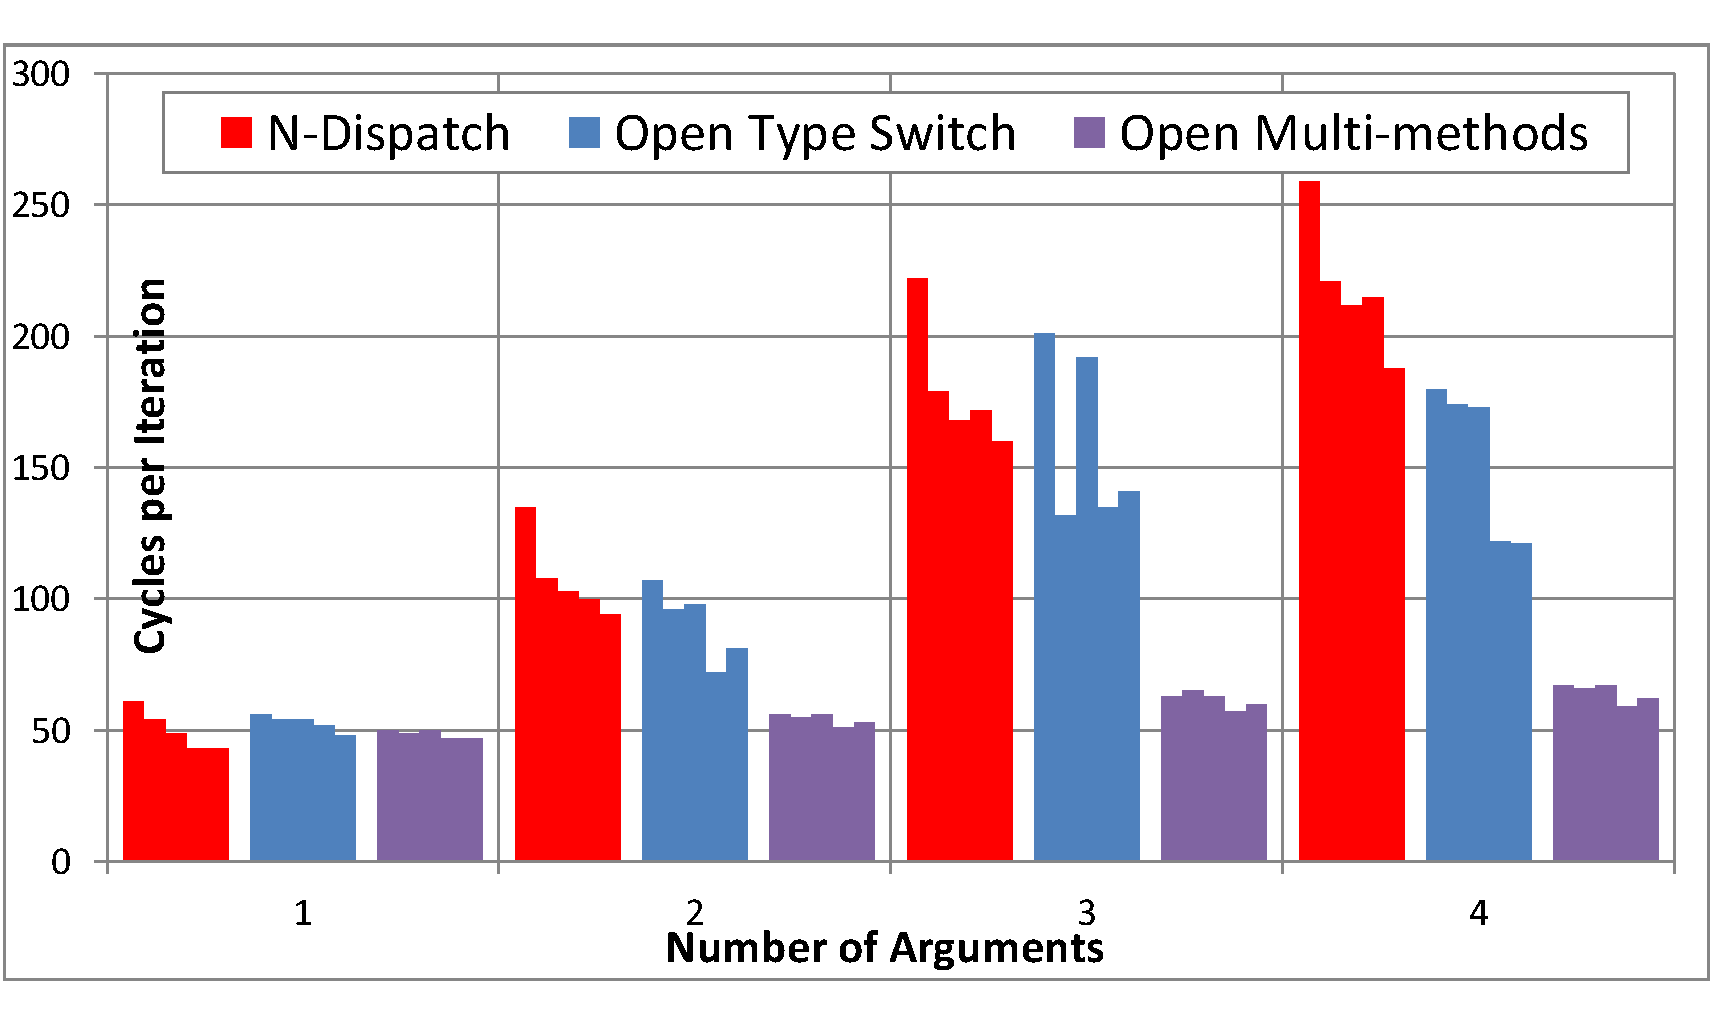
\includegraphics[width=0.49\textwidth]{Timing-N-arg.pdf}
  \caption{N-argument \code{Match}-statement vs. visitor design pattern and open multi-methods}
  \label{fig:dispatch}
\end{figure}

Open multi-methods provide the fastest performance because the dispatch is 
implemented with an $N$-dimensional array lookup, requiring only $4N+1$ memory 
references before an indirect call. N-Dispatch provides the slowest solution, 
requiring $2N$ virtual function calls (accept/visit per each dimension). Open 
type switch falls in between the two, thanks to its efficient hashing combined 
with a jump table.

In terms of memory, given a class hierarchy of $n$ classes (or $n$ subobjects in 
the subobject graph to be more precise) and a multiple dispatch on $N$ arguments 
from it, all 3 solutions will require the memory proportional to $O\of{n^N}$. 
More specifically, if $\delta$ is the number of bytes used by a pointer, then 
each of the approaches will use:

\begin{itemize}
\setlength{\itemsep}{0pt}
\setlength{\parskip}{0pt}
\item Open Multi-Methods: $\delta\of{n^N+Nn+N}$
\item N-Dispatch: $\delta\of{n^N+n^{N-1}+\cdots+n^2+n}$
\item Open Type Switch: $\delta\of{\of{2N+3}n^N+N+7}$
\end{itemize}

\noindent
bytes of memory. In all 3 cases the memory counted represents the non-reusable 
memory specific to the implementation of a single function dispatched through 
$N$ polymorphic arguments. Note that $n$ is a variable here since new classes 
may be loaded at run-time through dynamic linking in all 3 solutions, while $N$ 
is a constant, representing the number of arguments to dispatch on.

The memory used by each approach is allocated at different stages. The memory 
used by the virtual tables involved in the N-dispatch solution as well as 
dispatch tables used by open multi-methods will be allocated at compile/link 
time and will be reflected in the size of the final executable. Open 
multi-methods might require additional allocations and/or recomputation at load 
time to account for dynamic linking. In both cases, the memory allocated covers 
all possible combinations of $n$ classes in $N$ argument positions. In case of 
open type switch, the memory is only allocated at run-time and grows proportionally 
to the number of actual argument combinations seen by the type switch 
(\textsection\ref{sec:multiarg}). Only in the worst case when all possible 
combinations have been seen by the type switch does it reach the size described 
by the above formula. This is an important distinction as in many applications 
all-possible combinations will never be seen: for example, in a compiler the 
entities representing expressions and types might all be derived from a common 
base class, however they will rarely appear in the same type switch together.

There is also a significant difference in the ease of use of these solutions. 
N-Dispatch is the most restrictive solution as it is intrusive (and thus cannot 
be applied retroactively), hinders extensibility (by limiting the set of 
distinguishable cases) and is surprisingly hard to teach students. While 
analyzing Java idioms used to emulate multiple dispatch in practice, Muschevici 
et al~\cite[Figure 13]{MPTN08} noted that there are significantly more uses of 
cascading \code{instanceof} in the real code than the uses of double dispatch, 
which they also attribute to the obscurity of the second idiom. Both N-Dispatch 
and open multi-methods also introduce control inversion in which the case 
analysis is effectively structured in the form of callbacks. Open multi-methods 
are also subject to ambiguities, which have to be resolved at compile time and 
in some cases might require the addition of numerous overriders. Neither is the 
case with open type switch where the case analysis is performed directly, while 
ambiguities are avoided by the use of first-fit semantics.

%Although instanceof cascades may be slower than
%double dispatching, and are certainly less extensible, by
%being localised to a single class they are signi?cantly more
%straightforward to code than double dispatching. This may
%account for the relative popularity of each idiom.


\subsection{Rewriting Haskell code in \Cpp{}}
\label{sec:qualcmp}

For this experiment we took an existing code in Haskell and asked its author to 
rewrite it in \Cpp{} with \emph{Mach7}. The code in question is a simple 
peephole optimizer for an experimental GPU language called 
\emph{Versity}~\cite{Versity}. We assisted the author along the way to see which 
patterns he uses and what kind of mistakes he makes.

Somewhat surprising to us we found out that pattern-matching clauses generally 
became shorter, but their right-hand side became longer. The shortening of case 
clauses was perhaps specific to this application and mainly stemmed from the 
fact that Haskell does not support equivalence patterns or equivalence 
combinator and had to use guards to relate different arguments. This was 
particularly cumbersome when optimizer was looking at several arguments of 
several instructions in the stream, e.g.:

\begin{lstlisting}[language=Haskell]
peep2 (x1:x2:xs) = 
  case x1 of
    InstMove a b -> 
      case x2 of
        InstMove c d | (a == d) && (b == c) -> peep2 $ x1:xs
  ...
\end{lstlisting}

\noindent compared to \emph{Mach7} version:

\begin{lstlisting}
  Match(*x1,*x2) {
    Case(C<InstMove>(a,b), C<InstMove>(+b,+a)) ...
  ...
\end{lstlisting}

\noindent
Haskell also requires to use wildcard pattern in every unused position of a 
constructor pattern (e.g. \codehaskell{InstBin _ _ _ _}), while \emph{Mach7} 
allows one to omit all the trailing wildcards in constructor patterns (e.g. 
\code{C<InstBin>()}). And while this pays off only for constructor patterns with 
at least 3 arguments, the use of named patterns avoided many repeated pattern 
expressions and actually improved both performance and readability:

\begin{lstlisting}[columns=flexible]
  auto either = val(src) || val(dst);
  Match(inst) {
    Case(C<InstMove>(_,       either)) ...
    Case(C<InstUn>  (_, _,    either)) ...
    Case(C<InstBin> (_, _, _, either)) ...
  } EndMatch
\end{lstlisting}

\noindent
The disadvantage for \emph{Mach7} was coming after pattern matching, as we had to 
explicitly manage memory when inserting, removing or replacing instructions in 
the stream as well as explicitly manage the stream itself. Eventually we could 
hide some of this boilerplate behind smart pointers and other standard library 
classes.

During the initial rewrite into \Cpp{} the developer simply mapped Haskell 
patterns into their \emph{Mach7} equivalents, at which point we intervened and 
showed how some of the patterns can be expressed simpler. We reiterated the 
process until we could not improve the patterns ourselves without getting into 
the details of the actual simplifier. At one point we noticed that the developer 
started passing data via pattern-matching variables \code{var<T>} in and out of 
functions, which was not the intended use. This was hard to prevent statically, 
because in general, as first-class citizens, patterns can be passed in and out 
of functions, however in this case they were not used as patterns, but rather as 
values.

We have yet to make a performance comparison, but based on the performance of 
the open type switch~\cite{TS12} and the small overhead of our patterns, we 
expect the performance to be comparable.